\documentclass[11pt]{article}
% Switch [review] to [preprint] for a non-anonymous arXiv version, [final] for camera-ready.
\usepackage[review]{acl}
\usepackage{times}
\usepackage{latexsym}
\usepackage[T1]{fontenc}
\usepackage[utf8]{inputenc}
\usepackage{microtype}
\IfFileExists{inconsolata.sty}{\usepackage{inconsolata}}{}
\usepackage{graphicx}
% Shared macros. Placeholders are red so nothing slips into a submission.
\usepackage{xcolor}
\usepackage{booktabs,multirow,array,amsmath,amssymb,url}
\usepackage{pgfplots}
\usepackage{tikz}
\usepgfplotslibrary{groupplots}
\pgfplotsset{compat=1.17}
\usetikzlibrary{patterns,arrows.meta,positioning,shapes.geometric,fit,calc}

\newcommand{\xx}{\textcolor{red}{\textbf{XX}}}            % numeric placeholder
\newcommand{\todo}[1]{\textcolor{blue}{[TODO: #1]}}        % instruction to the runner
\newcommand{\phfig}{\node[rotate=22,gray!70,font=\large\bfseries] at (rel axis cs:0.5,0.5) {PLACEHOLDER};}
\newcommand{\bluff}{\textsc{BLUFF}}

% Colour-blind-safe palette for placeholder plots
\definecolor{cA}{HTML}{1B6CA8}
\definecolor{cB}{HTML}{D55E00}
\definecolor{cC}{HTML}{009E73}
\definecolor{cD}{HTML}{6C6C6C}


\title{Can Weight-Space Programming Fix the Long Tail?\\
A Position on Autonomous and Expert-in-the-Loop Model Surgery}

\author{Jason S. Lucas \\
  Secure and Ethical AI Lab (SEAL), Department of Information Science \\
  University of Colorado Boulder \\
  \texttt{jason.lucas@colorado.edu} \\\And
  Collaborator XX \\
  Affiliation XX}

\begin{document}
\maketitle

\begin{abstract}
Long-tail effects, meaning worse behavior on rare languages, dialects, and facts, arise at every stage of the model pipeline, and the standard repairs either need new training or risk damaging what the model already does well. We argue that \emph{weight-space programming}, in which a general LLM reads and writes a model's weights as text with no gradients \citep{takehi2026weightspace}, should be treated as a serious candidate repair for one class of long-tail failures: those where the model already holds the signal but something blocks it. We state four positions: (P1) the right question is whether a failure is an obstacle or a missing capability; (P2) surgery is cheaper and less damaging than editing and retraining for obstacles, and useless for missing capabilities; (P3) autonomy should be graded, with human review scaled to risk; and (P4) the same capability is dual-use, so evaluations must include it. We back the argument with a literature synthesis and pilot evidence from \bluff{} (78 languages, 20 big-head, 58 long-tail), and we give a research agenda.
\end{abstract}

\section{Introduction}
A model trained on unevenly distributed data behaves unevenly. On \bluff{}, detectors lose up to 25.3\% F1 on long-tail languages relative to big-head ones \citep{lucas2026bluff}. Rare facts are learned poorly \citep{kandpal2023longtail}, adding languages dilutes capacity \citep{conneau2020xlmr,chang2024curse}, and tokenization charges some languages up to 15 times more \citep{petrov2023tokenizers}. Fixing this at the source, with better data and larger models, is slow and expensive.

Repairs applied to a trained model are cheaper but have costs. Retraining or adapters need a run per language \citep{pfeiffer2020madx}. Merging needs compatible checkpoints \citep{ilharco2023task,tao2024merging}. Knowledge editors target facts, and sequential edits can collapse general ability \citep{meng2022rome,meng2023memit,zhang2026revive}. Neuron-level language interventions are cheap, but may not help low-resource transfer \citep{tang2024lape,mondal2025neurons}.

Weight-space programming proposes a different repair path \citep{takehi2026weightspace}. On Qwen3.5-0.8B, an LLM removed a single looping direction (0.016\% of weights, 50 forward passes) and raised MATH-500 from 7.9\% to 48.1\%; on Gemma 3 270M it gained nothing. The evidence is a single blog post, at up to 0.8B parameters, and not peer reviewed. We think the idea is promising enough, and risky enough, to deserve a position now, as long as the claims are tied to what the evidence can bear.

\section{Positions}
\label{sec:positions}
\begin{description}\itemsep2pt
\item[P1: Diagnose before you repair.] Long-tail failures split into \emph{obstacles} (the representation carries the signal, but a downstream component blocks it) and \emph{missing capabilities} (the signal is absent). Evaluations of repair methods should report which kind of failure they target.
\item[P2: Surgery is for obstacles.] For obstacles, an LLM-driven edit can be cheaper and less disruptive than retraining or fact editing. For missing capabilities, no edit helps; data or training is required.
\item[P3: Grade the autonomy.] Surgeons should operate on an explicit ladder from human-only to autonomous-with-veto, with regression suites, audit trails, rollback, and native-speaker sign-off scaled to risk.
\item[P4: Evaluate the misuse side.] The same capability can weaken safeguards or flip detectors. Open-weight release evaluations should include an autonomous-editor condition, reported in aggregate and by language.
\end{description}

\section{Long-Tail Effects Across the Pipeline}
\label{sec:pipeline}
Table~\ref{tab:pipeline} places long-tail causes by pipeline stage and says where surgery fits. The fit is a hypothesis to test, not a finding.

\begin{table*}[t]
\centering\small
\begin{tabular}{p{1.8cm} p{4.2cm} p{4.0cm} p{4.4cm}}
\toprule
Stage & Typical long-tail cause & Current repair & Surgery fit (hypothesis) \\
\midrule
Pretraining & Capacity dilution, tokenizer cost, thin data \citep{conneau2020xlmr,chang2024curse,petrov2023tokenizers} & Data mixing, larger models, tokenizer redesign & Low: causes are in data and tokens. Surgery may repair obstacles in released checkpoints \\
Post-training & Uneven safety and instruction coverage across languages \citep{yong2023lowresource,deng2024multijail} & Multilingual alignment data, safety-neuron tuning \citep{zhang2026safetyneurons,liang2026sparse} & Medium: targeted weight edits already show promise, so an LLM editor is a natural next step \\
Fine-tuning & Negative interference, forgetting, side effects of benign tuning \citep{biderman2024lora,qi2024finetuning} & Adapters, merging, LoRA & High: small, targeted edits with regression guards, as tested in our pilot \\
\bottomrule
\end{tabular}
\caption{Where long-tail effects arise and where weight surgery might help.}
\label{tab:pipeline}
\end{table*}

\section{Obstacle or Missing Capability?}
\label{sec:diag}
Figure~\ref{fig:quad} states the distinction. A model may represent a signal well or poorly, and its head may use it well or poorly. Only the cell where the representation is good and the readout is poor is repairable by edits that change weights without adding information.

\begin{figure}[t]
\centering
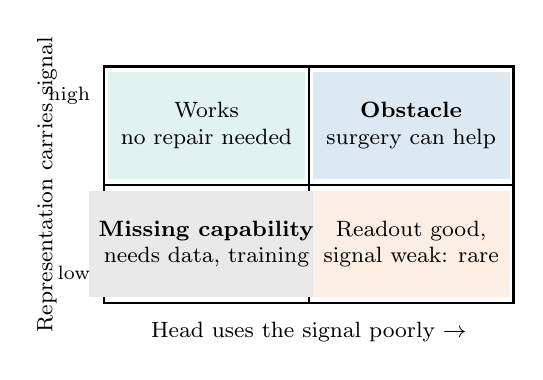
\begin{tikzpicture}[font=\footnotesize, x=2.6cm, y=1.5cm]
\draw[thick] (0,0) rectangle (2,2);
\draw[thick] (1,0) -- (1,2); \draw[thick] (0,1) -- (2,1);
\node[align=center, fill=cA!15, minimum width=2.5cm, minimum height=1.35cm] at (1.5,1.5) {\textbf{Obstacle}\\surgery can help};
\node[align=center, fill=cC!12, minimum width=2.5cm, minimum height=1.35cm] at (0.5,1.5) {Works\\no repair needed};
\node[align=center, fill=cD!15, minimum width=2.5cm, minimum height=1.35cm] at (0.5,0.5) {\textbf{Missing capability}\\needs data, training};
\node[align=center, fill=cB!10, minimum width=2.5cm, minimum height=1.35cm] at (1.5,0.5) {Readout good,\\signal weak: rare};
\node[rotate=90] at (-0.28,1) {Representation carries signal};
\node at (1,-0.25) {Head uses the signal poorly $\rightarrow$};
\node[font=\scriptsize, anchor=east] at (-0.02,1.75) {high};
\node[font=\scriptsize, anchor=east] at (-0.02,0.25) {low};
\end{tikzpicture}
\caption{Conceptual map. We operationalize the vertical axis with a linear probe on frozen features and the horizontal axis with the model's own head, so that obstacle score $o(\ell)=F_1^{\text{probe}}-F_1^{\text{head}}$.}
\label{fig:quad}
\end{figure}

The Gemma 3 270M result \citep{takehi2026weightspace} is the single data point we have for the lower row. The probe-based score is a practical way to sort real cases: it uses only a few labeled examples and a forward pass. Section~\ref{sec:pilot} gives our pilot test of whether it predicts which languages benefit.

\section{An Autonomy Ladder}
\label{sec:ladder}
Automated agents that experiment on other models exist \citep{rottshaham2024maia}, and so do the failure modes: confirmation bias and premature conclusions from thin evidence. We therefore propose four levels, each with a stated control (Table~\ref{tab:ladder}).

\begin{table*}[t]
\centering\small
\begin{tabular}{l p{3.6cm} p{4.6cm} p{4.2cm}}
\toprule
Level & Who acts & Required controls & Suitable for \\
\midrule
L0 & Human expert only & Regression suite, version control & Safety-critical changes, new model families \\
L1 & Surgeon proposes, human applies & Proposal diff, expert approval of each edit & Early deployment of the method \\
L2 & Surgeon applies, human reviews each edit & Automatic guard and rollback, review queue & Routine obstacle repairs \\
L3 & Surgeon runs to budget, human holds a veto & Guard, audit log, native-speaker sign-off, spot audits & Well-characterized repairs in low-risk domains \\
\bottomrule
\end{tabular}
\caption{Autonomy ladder. Moving up requires evidence from the level below (Section~\ref{sec:pilot}).}
\label{tab:ladder}
\end{table*}

Three controls are common to L1 through L3. A \emph{regression suite} covers languages and tasks the surgeon was not asked to change and includes a spectral check on edited matrices, since general ability tracks dominant singular directions \citep{zhang2026revive}. An \emph{audit trail} records every proposal, edit, metric, and rollback. \emph{Native-speaker sign-off} gates any change that claims to help a language community, because automatic metrics can miss harm.

\section{Pilot Evidence}
\label{sec:pilot}
We report three pilots. Each is deliberately small and exists to show that the argument can be tested, not to settle it. \todo{Replace XX and placeholder figures with runs; Pilot 1 reuses Paper 1 outputs.}

\paragraph{Pilot 1: fine-tuning stage on \bluff{}.}
On \bluff{} (78 languages: 20 big-head, 58 long-tail), surgery reduces the big-head versus long-tail gap from \xx{} to \xx{} F1 points, and gains rise with the obstacle score (Spearman $\rho=\xx{}$; Figure~\ref{fig:pilot}a).

\paragraph{Pilot 2: post-training stage.}
On \xx{} open chat models, we compare the aggregate refusal-rate gap between high- and low-resource languages before and after a surgeon-proposed repair that is applied only to the safety-strengthening direction. The gap narrows from \xx{} to \xx{} points with \xx{} points of capability change.

\paragraph{Pilot 3: expert in the loop.}
Table~\ref{tab:human} compares autonomy levels with \xx{} expert participants (ML engineers and native-speaker reviewers) on matched repairs: time to fix, success, regressions, and review burden.

\begin{table}[t]
\centering\small\setlength{\tabcolsep}{3.5pt}
\begin{tabular}{l rrrr}
\toprule
Level & Succ.\ \% & Regr. & Exp.\ min. & Rej. \\
\midrule
L0 Human only & \xx & \xx & \xx & \xx \\
L1 Proposes & \xx & \xx & \xx & \xx \\
L2 Applies, rev. & \xx & \xx & \xx & \xx \\
L3 Auton. + veto & \xx & \xx & \xx & \xx \\
\bottomrule
\end{tabular}
\caption{Expert-in-the-loop pilot. Regr.\ counts regressions found by the suite; Rej.\ counts edits a native-speaker reviewer rejected.}
\label{tab:human}
\end{table}

\begin{figure}[t]
\centering
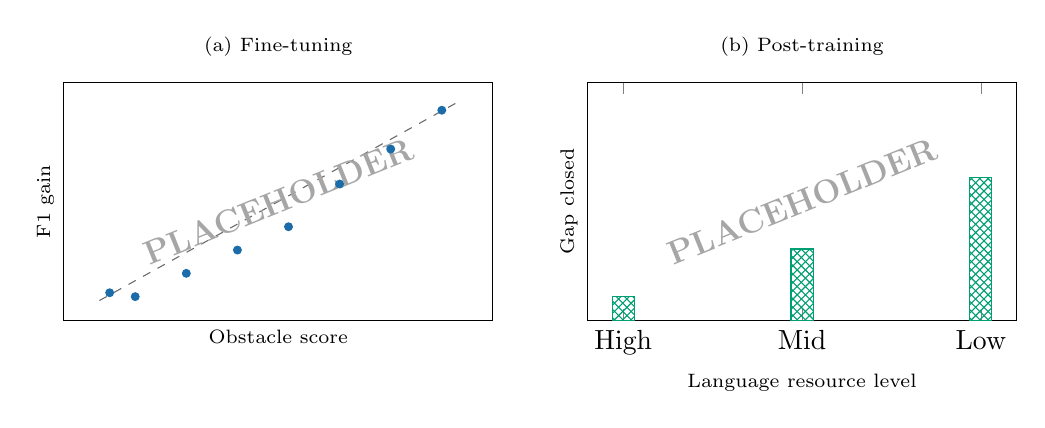
\begin{tikzpicture}
\begin{groupplot}[group style={group size=2 by 1, horizontal sep=1.2cm}, width=0.58\columnwidth, height=4.6cm,
  xticklabels={}, yticklabels={}, xtick=\empty, ytick=\empty, label style={font=\scriptsize}, title style={font=\scriptsize}]
\nextgroupplot[xlabel={Obstacle score}, ylabel={F1 gain}, title={(a) Fine-tuning}]
\addplot[only marks, mark=*, cA, mark size=1.4pt] coordinates {(0.5,0.3) (1,0.2) (2,0.8) (3,1.4) (4,2.0) (5,3.1) (6,4.0) (7,5.0)};
\addplot[dashed, cD, no marks] coordinates {(0.3,0.1) (7.3,5.2)};
\phfig
\nextgroupplot[xlabel={Language resource level}, ylabel={Gap closed}, title={(b) Post-training}, symbolic x coords={High,Mid,Low}, xtick=data, ymin=0, ymax=1]
\addplot[ybar, fill=white, draw=cC, pattern=crosshatch, pattern color=cC, bar width=8pt] coordinates {(High,0.1) (Mid,0.3) (Low,0.6)};
\phfig
\end{groupplot}
\end{tikzpicture}
\caption{Placeholder: (a) gain versus obstacle score (claim: positive relation); (b) share of the high versus low-resource refusal gap closed by a targeted repair, by resource level (claim: larger for the long tail).}
\label{fig:pilot}
\end{figure}

\section{Alternative Views}
\label{sec:alt}
\paragraph{``Just retrain or add data.''} For missing capabilities this is right (P2), and we expect most deep long-tail failures to be of this kind \citep{kandpal2023longtail}. Surgery is a complement for the obstacle subset, and the diagnostic is how to tell the cases apart.

\paragraph{``Editing already does this.''} Editors target facts and can degrade general ability with repeated edits \citep{meng2023memit,zhang2026revive}. Surgery inherits that risk, which is why we require regression suites and spectral guards. Whether an LLM editor improves on ROME-style methods for language failures is an empirical question, and Pilot 1 includes them as baselines.

\paragraph{``The evidence is one blog post.''} Agreed, and the scale tested is under one billion parameters. We treat the result as a hypothesis and propose tests, including negative controls, that could refute it.

\paragraph{``This makes tampering easy.''} Single-direction and fine-tuning attacks already exist \citep{arditi2024refusal,qi2024finetuning}. The new question is the marginal effect of autonomy, which a companion study measures in aggregate. Restricting the capability would also remove a tool for language communities, so we favor evaluation and disclosure over prohibition.

\section{Governance}
\label{sec:gov}
We recommend that (i) release evaluations for open-weight models include an autonomous-editor condition reported by language group, (ii) repairs that claim to help a language community carry native-speaker sign-off, (iii) tamper-resistance claims \citep{tamirisa2025tar} be tested against agent edits, and (iv) audit logs be retained so that any edit can be reviewed and reversed.

\section{Research Agenda}
\label{sec:agenda}
\begin{enumerate}\itemsep0pt
\item Replicate the original result at larger scale and on multiple surgeons.
\item Validate the obstacle score against interventions that cannot add information, across tasks and not only detection.
\item Establish regression suites for languages, including spectral checks and generation quality.
\item Measure marginal misuse risk under controlled release, and test weight-only auditors on agent edits.
\item Study when native-speaker review is needed and how to make it cheap.
\end{enumerate}

\section*{Limitations}
This is a position paper with pilot evidence. The method is supported by one non-peer-reviewed report at up to 0.8B parameters, the pilots are small, and the obstacle score is a proxy. Tokenizer disparity and missing knowledge are outside the reach of weight edits.

\section*{Ethics Statement}
The position includes a dual-use discussion and a governance proposal. No procedures for removing safeguards are given, and aggregate results only are reported from the companion safety study.

\section*{Acknowledgments}
\todo{Funding, reviewers, collaborators.}

\bibliography{references}
\end{document}
